% fig_transit_times.tex - Transit time comparison plot
% Standalone compilation: pdflatex fig_transit_times.tex
\documentclass[tikz,border=5pt]{standalone}
\usepackage{pgfplots}
\usepackage{amsmath}
\pgfplotsset{compat=1.18}

\begin{document}
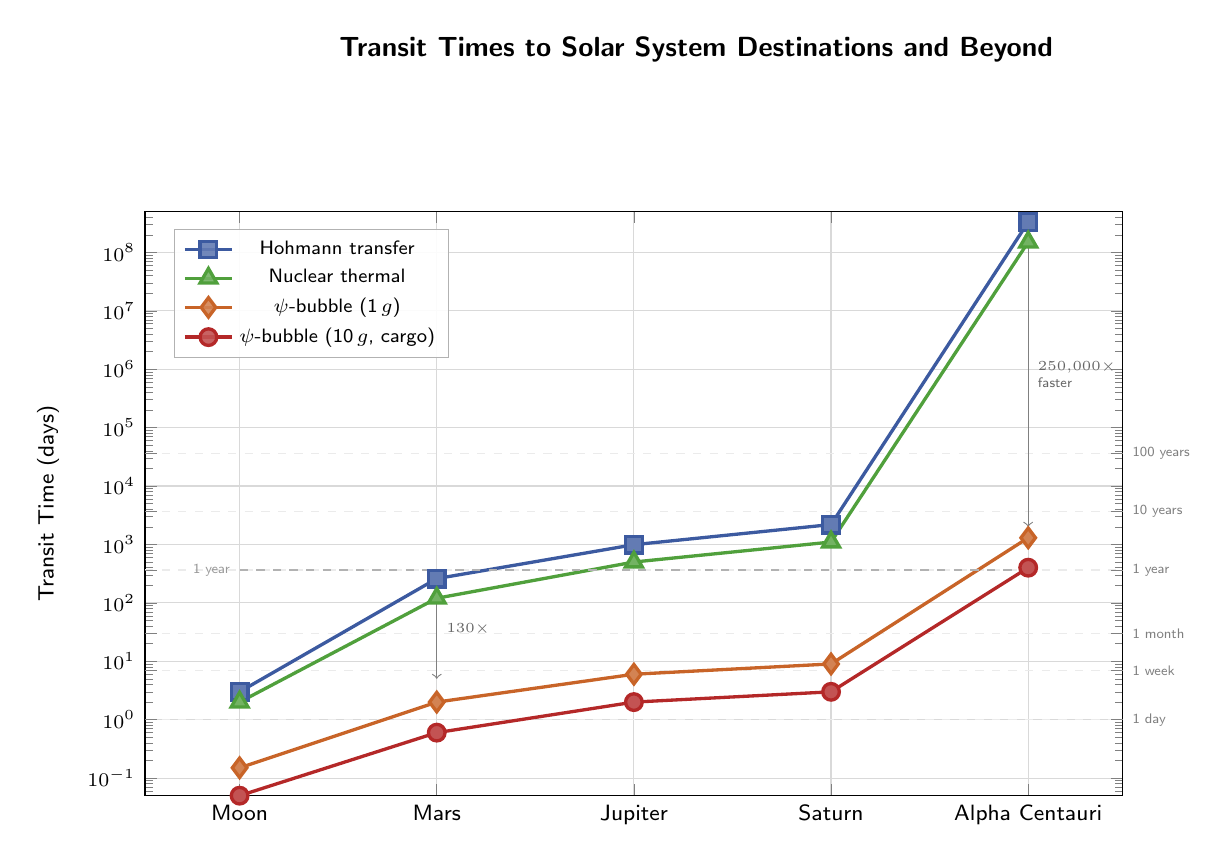
\begin{tikzpicture}

\definecolor{hohmann}{RGB}{60,90,160}
\definecolor{nucth}{RGB}{80,160,60}
\definecolor{psi1g}{RGB}{200,100,40}
\definecolor{psi10g}{RGB}{180,40,40}

\begin{axis}[
    width=14cm, height=9cm,
    ymode=log,
    ymin=0.05, ymax=5e8,
    ylabel={Transit Time (days)},
    ylabel style={font=\footnotesize\sffamily},
    xlabel style={font=\footnotesize\sffamily},
    tick label style={font=\scriptsize\sffamily},
    symbolic x coords={Moon, Mars, Jupiter, Saturn, {Alpha Centauri}},
    xtick=data,
    x tick label style={font=\footnotesize\sffamily},
    enlarge x limits=0.12,
    grid=major,
    grid style={black!15},
    legend style={
        font=\scriptsize\sffamily,
        at={(0.03,0.97)},
        anchor=north west,
        draw=black!30,
        fill=white,
        fill opacity=0.9,
        text opacity=1,
    },
    % Extra y-axis ticks for time scale reference
    extra y ticks={1, 7, 30, 365, 3650, 36500},
    extra y tick labels={1 day, 1 week, 1 month, 1 year, 10 years, 100 years},
    extra y tick style={
        grid=major,
        grid style={black!8, dashed},
        tick label style={font=\tiny\sffamily, text=black!50, anchor=west},
        ticklabel pos=right,
    },
]

% --- Hohmann transfer ---
\addplot[
    color=hohmann, very thick, mark=square*, mark size=3pt,
    mark options={fill=hohmann!80},
] coordinates {
    (Moon, 3)
    (Mars, 260)
    (Jupiter, 990)
    (Saturn, 2190)
    (Alpha Centauri, 3.3e8)
};
\addlegendentry{Hohmann transfer}

% --- Nuclear thermal ---
\addplot[
    color=nucth, very thick, mark=triangle*, mark size=3.5pt,
    mark options={fill=nucth!80},
] coordinates {
    (Moon, 2)
    (Mars, 120)
    (Jupiter, 500)
    (Saturn, 1100)
    (Alpha Centauri, 1.5e8)
};
\addlegendentry{Nuclear thermal}

% --- Psi-bubble at 1g ---
\addplot[
    color=psi1g, very thick, mark=diamond*, mark size=3.5pt,
    mark options={fill=psi1g!80},
] coordinates {
    (Moon, 0.15)
    (Mars, 2)
    (Jupiter, 6)
    (Saturn, 9)
    (Alpha Centauri, 1300)
};
\addlegendentry{$\psi$-bubble (1\,$g$)}

% --- Psi-bubble at 10g ---
\addplot[
    color=psi10g, very thick, mark=*, mark size=3pt,
    mark options={fill=psi10g!80},
] coordinates {
    (Moon, 0.05)
    (Mars, 0.6)
    (Jupiter, 2)
    (Saturn, 3)
    (Alpha Centauri, 400)
};
\addlegendentry{$\psi$-bubble (10\,$g$, cargo)}

% --- Annotations for dramatic comparisons ---
% Mars
\draw[->, black!50, thin] (axis cs:Mars,260) -- (axis cs:Mars,5)
    node[midway, right, font=\tiny\sffamily, text=black!60] {$130\times$};

% Alpha Centauri
\draw[->, black!50, thin] (axis cs:{Alpha Centauri},3.3e8) -- (axis cs:{Alpha Centauri},2000)
    node[midway, right, font=\tiny\sffamily, text=black!60, align=left]
    {$250{,}000\times$\\faster};

% Human tolerance line
\draw[black!30, dashed, thick] (axis cs:Moon,365) -- (axis cs:{Alpha Centauri},365);
\node[font=\tiny\sffamily, text=black!40, anchor=east] at (axis cs:Moon,365) {1 year};

\end{axis}

% ============================================================
% TITLE
% ============================================================
\node[font=\normalsize\sffamily\bfseries, anchor=south] at (7,9.2)
    {Transit Times to Solar System Destinations and Beyond};

\end{tikzpicture}
\end{document}
